\documentclass[a4]{article}
\pagestyle{myheadings}

%%%%%%%%%%%%%%%%%%%
% Packages/Macros %
%%%%%%%%%%%%%%%%%%%
\usepackage{mathrsfs}


\usepackage{fancyhdr}
\pagestyle{fancy}
\lhead{}
\chead{}
\rhead{}
\lfoot{}
\cfoot{} 
\rfoot{\normalsize\thepage}
\renewcommand{\headrulewidth}{0pt}
\renewcommand{\footrulewidth}{0pt}
\newcommand{\RomanNumeralCaps}[1]
    {\MakeUppercase{\romannumeral #1}}

\usepackage{amssymb,latexsym}  % Standard packages
\usepackage[utf8]{inputenc}
\usepackage[russian]{babel}
\usepackage{MnSymbol}
\usepackage{mathrsfs}
\usepackage{amsmath,amsthm}
\usepackage{indentfirst}
\usepackage{graphicx}%,vmargin}
\usepackage{graphicx}
\graphicspath{{pictures/}} 
\usepackage{verbatim}
\usepackage{color}
\usepackage[nottoc,numbib]{tocbibind}
\usepackage{float}

\usepackage{listings}
\definecolor{codegreen}{rgb}{0,0.6,0}
\definecolor{codegray}{rgb}{0.5,0.5,0.5}
\definecolor{codepurple}{rgb}{0.58,0,0.82}
\definecolor{backcolour}{rgb}{0.95,0.95,0.92}
 
\lstdefinestyle{mystyle}{
    backgroundcolor=\color{backcolour},   
    commentstyle=\color{codegreen},
    keywordstyle=\color{magenta},
    numberstyle=\tiny\color{codegray},
    stringstyle=\color{codepurple},
    basicstyle=\footnotesize,
    breakatwhitespace=false,         
    breaklines=true,                 
    captionpos=b,                    
    keepspaces=true,                 
    numbers=left,                    
    numbersep=5pt,                  
    showspaces=false,                
    showstringspaces=false,
    showtabs=false,                  
    tabsize=2
}
 
\lstset{style=mystyle}

\usepackage{url}
\urldef\myurl\url{foo%.com}





\DeclareGraphicsExtensions{.pdf,.png,.jpg}% -- настройка картинок

\usepackage{epigraph} %%% to make inspirational quotes.
\usepackage[all]{xy} %for XyPic'a
\usepackage{color} 
\usepackage{amscd} %для коммутативных диграмм
%\usepackage[colorlinks,urlcolor=red]{hyperref}

%\renewcommand{\baselinestretch}{1.5}
%\sloppy
%\usepackage{listings}
%\lstset{numbers=left}
%\setmarginsrb{2cm}{1.5cm}{1cm}{1.5cm}{0pt}{0mm}{0pt}{13mm}


\newtheorem{Lemma}{Лемма}[section]
\newtheorem{Proposition}{Предложение}[section]
\newtheorem{Theorem}{Теорема}[section]
\newtheorem{Corollary}{Следствие}[section]
\newtheorem{Remark}{Замечание}[section]
\newtheorem{Definition}{Определение}[section]
\newtheorem{Designations}{Обозначение}[section]




%%%%%%%%%%%%%%%%%%%%%%% 
%Подготовка оглавления% 
%%%%%%%%%%%%%%%%%%%%%%% 
\usepackage[titles]{tocloft}
\renewcommand{\cftdotsep}{2} %частота точек
\renewcommand\cftsecleader{\cftdotfill{\cftdotsep}}
\renewcommand{\cfttoctitlefont}{\hspace{0.38\textwidth} \LARGE\bfseries} 
\renewcommand{\cftsecaftersnum}{.}
\renewcommand{\cftsubsecaftersnum}{.}
\renewcommand{\cftbeforetoctitleskip}{-1em} 
\renewcommand{\cftaftertoctitle}{\mbox{}\hfill \\ \mbox{}\hfill{\footnotesize Стр.}\vspace{-0.5em}} 
%\renewcommand{\cftchapfont}{\normalsize\bfseries \MakeUppercase{\chaptername} } 
%\renewcommand{\cftsecfont}{\hspace{1pt}} 
\renewcommand{\cftsubsecfont}{\hspace{1pt}} 
%\renewcommand{\cftbeforechapskip}{1em} 
\renewcommand{\cftparskip}{3mm} %определяет величину отступа в оглавлении
\setcounter{tocdepth}{5} 
\renewcommand{\listoffigures}{\begingroup %добавляем номер в список иллюстраций
\tocsection
\tocfile{\listfigurename}{lof}
\endgroup}
\renewcommand{\listoftables}{\begingroup %добавляем номер в список иллюстраций
\tocsection
\tocfile{\listtablename}{lot}
\endgroup}


   
   
%\renewcommand{\thelikesection}{(\roman{likesection})}
%%%%%%%%%%%
% Margins %
%%%%%%%%%%%
\addtolength{\textwidth}{0.7in}
\textheight=630pt
\addtolength{\evensidemargin}{-0.4in}
\addtolength{\oddsidemargin}{-0.4in}
\addtolength{\topmargin}{-0.4in}

%%%%%%%%%%%%%%%%%%%%%%%%%%%%%%%%%%%
%%%%%%Переопределение chapter%%%%%% 
%%%%%%%%%%%%%%%%%%%%%%%%%%%%%%%%%%%
\newcommand{\empline}{\mbox{}\newline} 
\newcommand{\likechapterheading}[1]{ 
\begin{center} 
\textbf{\MakeUppercase{#1}} 
\end{center} 
\empline} 

%%%%%%%Запиливание переопределённого chapter в оглавление%%%%%% 
\makeatletter 
\renewcommand{\@dotsep}{2} 
\newcommand{\l@likechapter}[2]{{\bfseries\@dottedtocline{0}{0pt}{0pt}{#1}{#2}}} 
\makeatother 
\newcommand{\likechapter}[1]{ 
\likechapterheading{#1} 
\addcontentsline{toc}{likechapter}{\MakeUppercase{#1}}} 




\usepackage{xcolor}
\usepackage{hyperref}
\definecolor{linkcolor}{HTML}{000000} % цвет ссылок
\definecolor{urlcolor}{HTML}{3643FF} % цвет гиперссылок
 
\hypersetup{pdfstartview=FitH,  linkcolor=linkcolor,urlcolor=urlcolor, colorlinks=true}

%%%%%%%%%%%%
% Document %
%%%%%%%%%%%%

%%%%%%%%%%%%%%%%%%%%%%%%%%%%%
%%%%%%главы -- section*%%%%%%
%%%%section -- subsection%%%%
%subsection -- subsubsection%
%%%%%%%%%%%%%%%%%%%%%%%%%%%%%
\def \newstr {\medskip \par \noindent} 



\begin{document}
\def\contentsname{\LARGE{Содержание}}
\thispagestyle{empty}
\begin{center} 
\vspace{2cm} 
{\Large \sc Санкт-Петербургский Политехнический}\\
\vspace{2mm}
{\Large \sc Университет} им. {\Large\sc Петра Великого}\\
\vspace{1cm}
{\large \sc Институт прикладной математики и механики\\ 
\vspace{0.5mm}
\textsc{}}\\ 
\vspace{0.5mm}
{\large\sc Кафедра прикладной математики}\\
\vspace{15mm}
%\rule[0.5ex]{\linewidth}{2pt}\vspace*{-\baselineskip}\vspace*{3.2pt} 
%\rule[0.5ex]{\linewidth}{1pt}\\[\baselineskip] 
{\huge \sc Лабораторная работа №$2$\\
	Боксплот Тьюки
	\vspace{6mm}
	
}
\vspace*{2mm}
%\rule[0.7ex]{\linewidth}{1pt}\vspace*{-\baselineskip}\vspace{3.2pt} 
%\rule[0.5ex]{\linewidth}{2pt}\\ 
\vspace{6cm} 
Студент группы $3630102/70301$ \hfill Камянский Д.В.\\
\vspace{1cm}
Преподаватель \hfill Баженов А. Н.\\
\vspace{20mm} 


\vfill {\large\textsc{Санкт-Петербург}}\\ 
2020 г.
\end{center}

%%%%%%%%%%%%%%%%%%%%%%%%%%%%%%%%%%%%%%%%%%%%%%%%%%%%%%%%%%%%%%%%%%%%%%%%%%%%%%%%%%%%%%%%%%%%%%
%\ \\[4cm]

%\rm
%%%%%%%%%%%%%%%%%%%%%%%%%%%%%%%%%%%%%%%%%%%%%%%%%%%%%%%%%%%%%%%%%%%%%%%%%%%%%%%%%%%%%%%%%%%%%%
\newpage
\pagestyle{plain}

%\begin{center}
%\begin{abstract} 

%\end{abstract}

%\end{center}

\newpage
\tableofcontents{}
\newpage
\listoffigures{}
\listoftables{}
\newpage

\section{Постановка задачи}

Для, приведённых ниже, пяти распределений сгенерировать выборки объёмом 20, 100, для каждой выборки построить боксплот Тьюки. Для каждого распределения экспериментально определить процент выбросов, сгенерировав выборку, соответствующую распределению $1000$ раз и, вычислив среднюю долю выбросов. Сравнить полученные оценки с результатами, полученными теоретически.


Распределения:
\begin{equation}\label{eqn:normal}
N(x,0,1) = \frac{1}{\sqrt{2\pi}}e^{-\frac{x^2}{2}}
\end{equation} 

\begin{equation}\label{eqn:cauchy}
C(x,0,1) = \frac{1}{\pi(1+x^2)}
\end{equation}

\begin{equation}\label{eqn:laplace}
L\left( x,0,\frac{1}{\sqrt{2}}\right) = \frac{1}{\sqrt{2}}e^{-\sqrt{2}\vert x\vert}
\end{equation}

\begin{equation}\label{eqn:poisson}
P(5,k) = \frac{5^k}{k!}e^{-5}
\end{equation}  

\begin{equation}\label{eqn:uniform}
M(x,-\sqrt{3}, \sqrt{3}) = 
\begin{cases}
\frac{1}{2\sqrt{3}} &\vert x\vert \leqslant \sqrt{3}\\
0 &\vert x\vert > \sqrt{3}
\end{cases}
\end{equation}



\section{Теория}

Боксплот Тьюки - график, использующийся в описательной статистике, изображающий одномерное распределение вероятностей.

Границами ящика служат первый и третий квартили, линия в середине
ящика — медиана. Концы усов — края статистически значимой выборки
(без выбросов). Длину «усов» определяют разность первого квартиля и полутора межквартильных расстояний и сумма третьего квартиля и полутора межквартильных расстояний. 

Выбросом в статистике называют результат измерения, выделяющийся из общей выборки.

Правая и левая границы:  $X_{1} = Q_{1} - 1.5(Q_{3} - Q_{1}),\;X_{2} = Q_{3} + 1.5(Q_{3} - Q_{1})$

Теоретическая вероятность выбросов:\\
Для непрерывных распределений:
$P^{t}_{e} = F(X_{1}^{t}) + (1 - F(X_{2}^{t}))$\\
Для дискретных распределений:
$P^{t}_{e} = (F(X_{1}^{t}) - P(x=X_{1}^{t})) + (1 - F(X_{2}^{t}))$

\section{Реализация}
Для генерации выборки был использован $Python\;3.8.2$: модуль $stats$ библиотеки $scipy$ для генерации выборок различных распределений.

Боксплот Тьюки был построен средствами библиотеки $seaborn$.

Число выбросов определялось таким образом: если значение из выборки находится вне установленных левой и правых границ, то оно является выбросом.


\newpage
\section{Результаты}
\begin{center}

\begin{figure}[H]
\caption{Boxplot распределений для размера выборки N=20 }
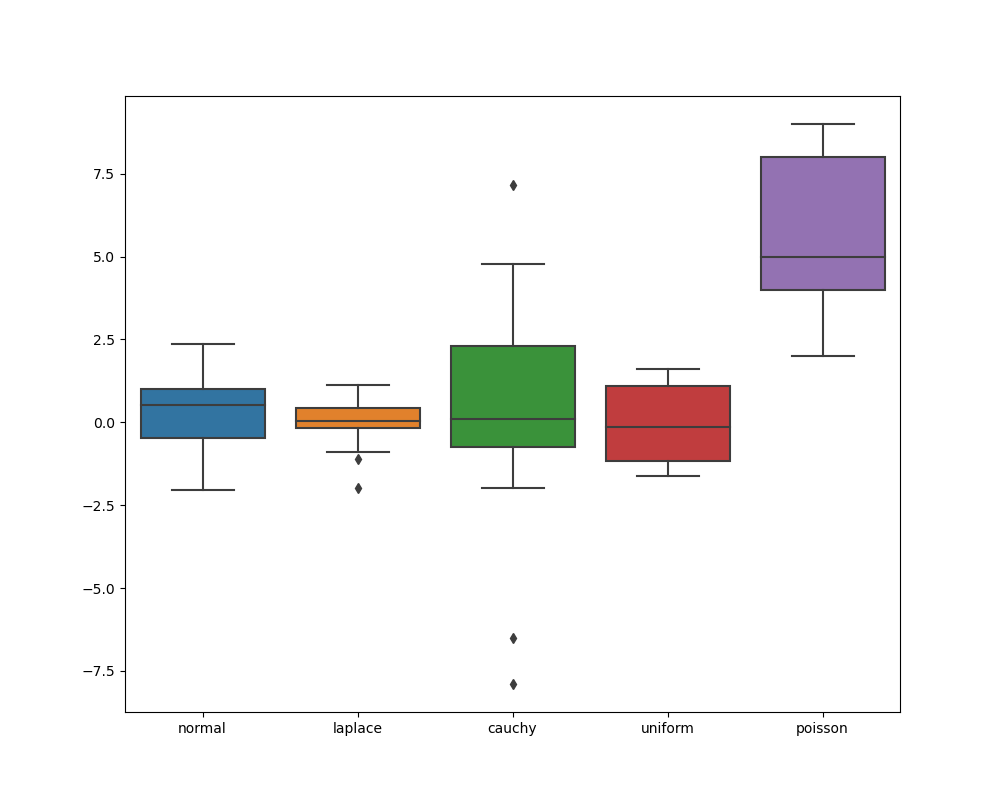
\includegraphics[width=\textwidth]{boxplot_N=20.png}
\end{figure}

\begin{figure}[H]
	\caption{Boxplot стандартное нормальное распределение }
	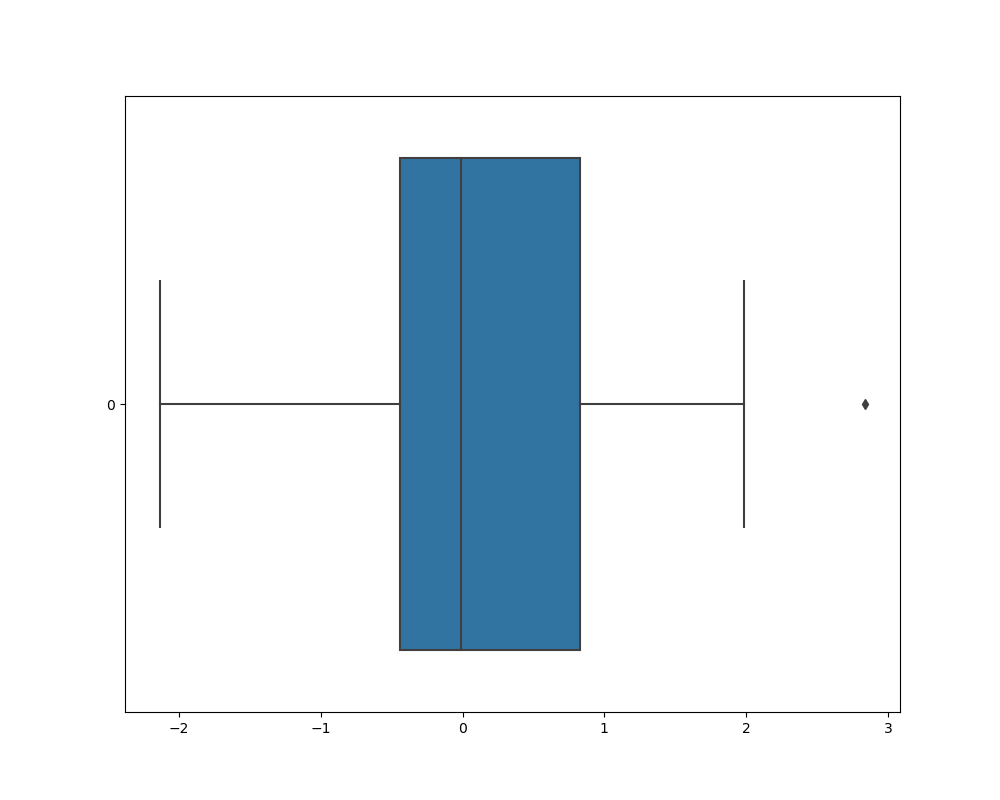
\includegraphics[width=\textwidth]{boxplot_N=100_normal.png} 
\end{figure}

\begin{figure}[H]
\caption{Boxplot стандартное распределение Лапласа }
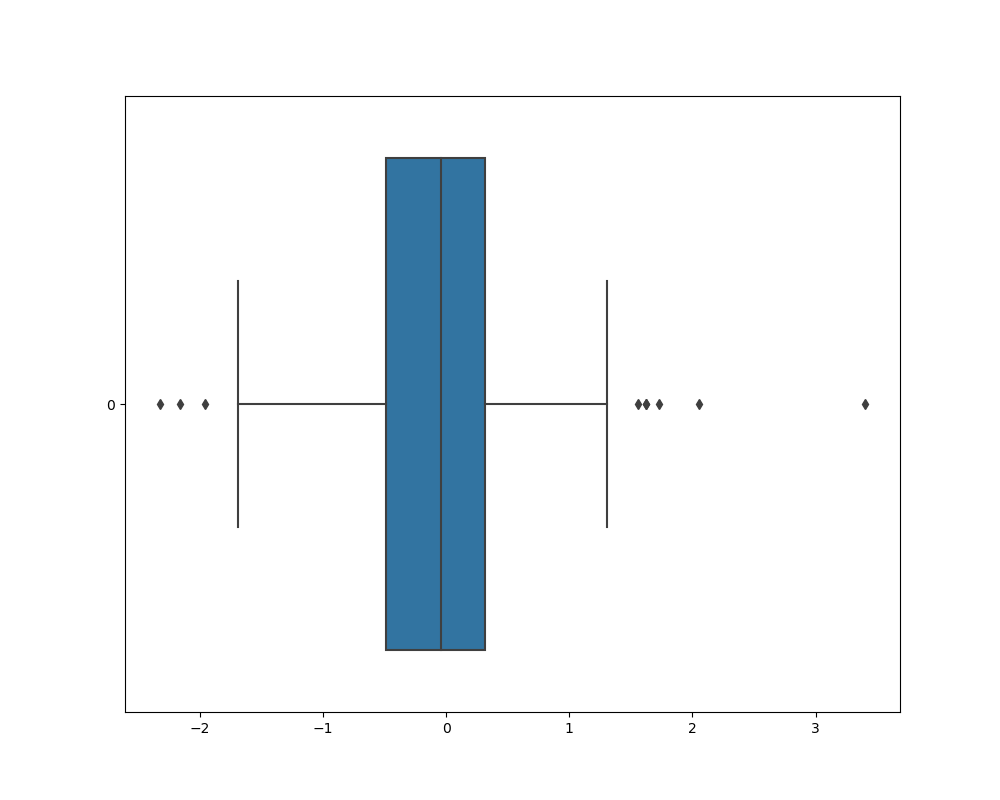
\includegraphics[width=\textwidth]{boxplot_N=100_laplace.png} 
\end{figure}

\begin{figure}[H]
\caption{Boxplot стандартное распределение Коши }
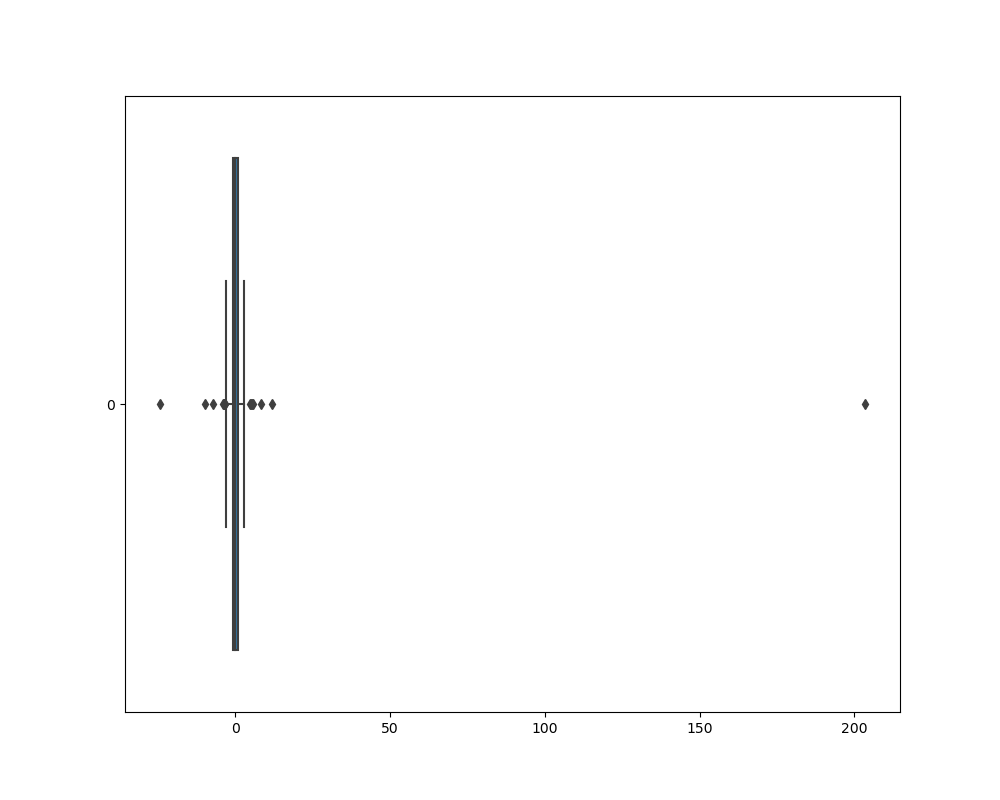
\includegraphics[width=\textwidth]{boxplot_N=100_cauchy.png} 
\end{figure}

\begin{figure}[H]
\caption{Boxplot распределение Пуассона }
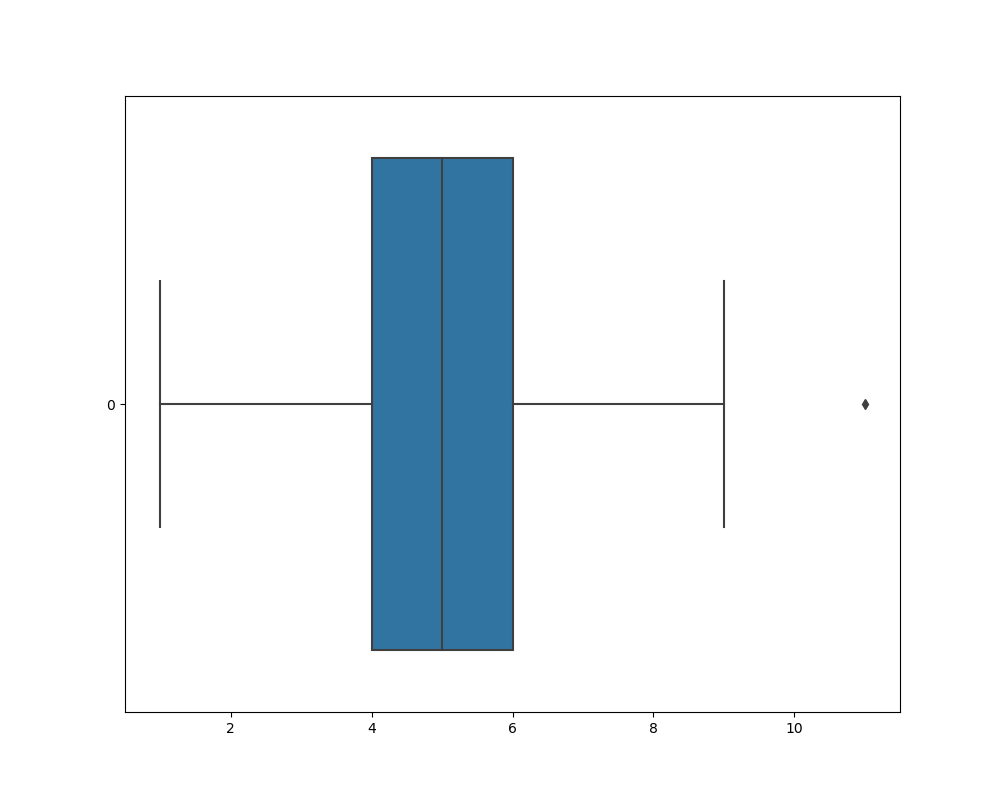
\includegraphics[width=\textwidth]{boxplot_N=100_poisson.png} 
\end{figure}

\begin{figure}[H]
 \caption{Boxplot равномерное распределение }
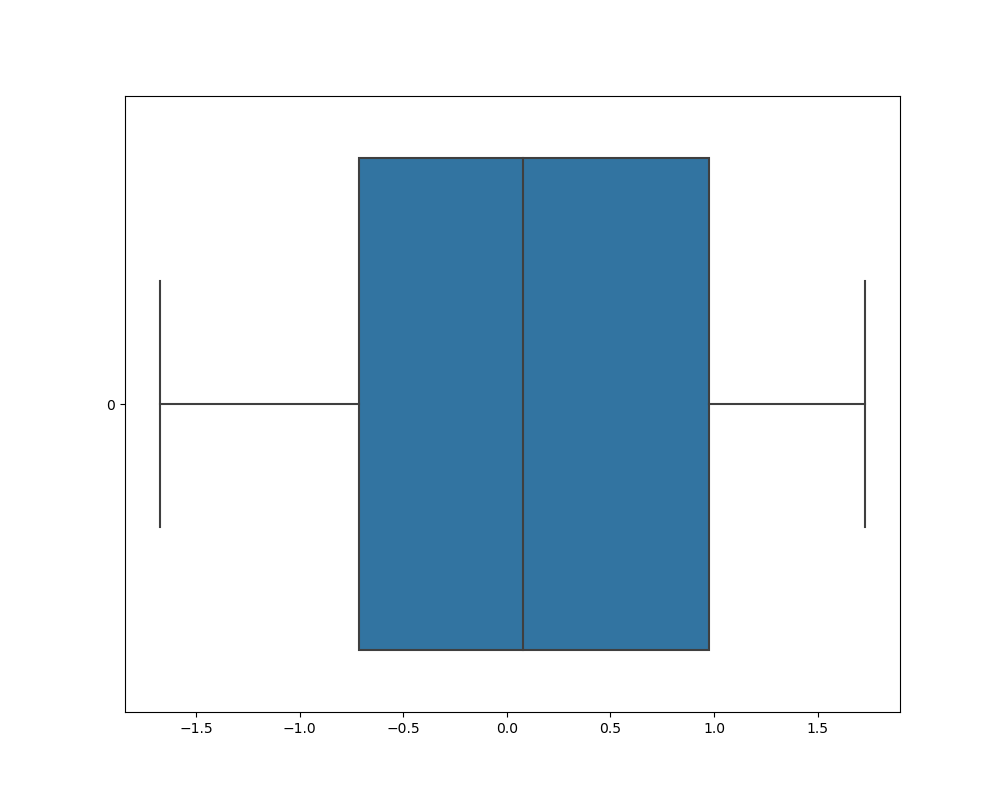
\includegraphics[width=\textwidth]{boxplot_N=100_uniform.png}
\end{figure}

\begin{table}[H]
    
    \caption{Эксперементальные оценки доли выбросов}
    \label{tab:my_label}
    \begin{center}
    \vspace{5mm}
    \begin{tabular}{|c|c|}
    \hline
    Распределение & Доля выбросов\\
    \hline
         normal	& 0.006977\\
         \hline
cauchy & 0.155958\\
\hline
laplace	& 0.0625\\
\hline
uniform	& 0.0\\
\hline
poisson	& 0.013695\\
\hline
    \end{tabular}
    
    \end{center}
    
\end{table}

\begin{table}[H]
	
	\caption{Теоретические оценки доли выбрасов}
	\label{tab:my_label}
	\begin{center}
		\vspace{5mm}
		\begin{tabular}{|c|c|}
			\hline
			Распределение & Доля выбросов\\
			\hline
			normal	&\\
			\hline
			n = 20   & 	0.02275    \\
			\hline
			n = 100   &	0.01036    \\
			\hline
			cauchy	&\\
			\hline
			n = 20   & 	0.1525    \\
			\hline
			n = 100  & 	0.15546    \\
			\hline
			laplace	&\\
			\hline
			n = 20    &	0.0735    \\
			\hline
			n = 100   &	0.06576    \\
			\hline
			uniform	&\\
			\hline
			n = 20    &	0.00135    \\
			\hline
			n = 100   &	0.0   \\ 
			\hline
			poisson	&\\
			\hline
			n = 20   & 	0.0264    \\
			\hline
			n = 100  & 	0.01478    \\
			\hline
		\end{tabular}
		
	\end{center}
	
\end{table}

\end{center}


\section{Выводы}
\par Экспериментально полученные оценки доли выбросов стремятся к теоретическим с ростом размера выборки.
Можно вывести соотношение между процентами выбросов:

\begin{equation}
uniform<normal<poisson<laplace<cauchy
\end{equation}

\par По полученным данным видно, что наименьший процент выбросов у равномерного распределения, а наибольший процент выбросов у распределения Коши, при чем значения этих выбросов могут отклонятся от выборочного среднего на порядки.

\begin{thebibliography}{}    
    \href{https://en.wikipedia.org/wiki/Box\_plot}{Боксплот}\\
    \href{https://docs.scipy.org/doc/scipy/reference/stats.html}{Модуль scipy.stats}\\
    \href{https://seaborn.pydata.org/}{Модуль seaborn}
\end{thebibliography}

\section{Приложения}


Код лаборатрной:\; \url{https://github.com/dkamianskii/MatStatLabs/tree/master/Lab3}


\end{document}